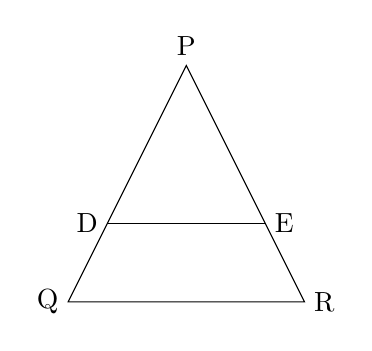
\begin{tikzpicture}[scale=1]
    % Triangle PQR
    \coordinate (P) at (1.5, 3);
    \coordinate (Q) at (0, 0);
    \coordinate (R) at (3, 0);
    \draw (P) -- (Q) -- (R) -- cycle;
    
    % Internal line DE parallel to QR
    \coordinate (D) at (0.5, 1);
    \coordinate (E) at (2.5, 1);
    \draw (D) -- (E);
    
    % Labels
    \node[above] at (P) {P};
    \node[left] at (Q) {Q};
    \node[right] at (R) {R};
    \node[left] at (D) {D};
    \node[right] at (E) {E};
\end{tikzpicture}